\documentclass[10pt,landscape]{article}
\usepackage{multicol}
\usepackage{calc}
\usepackage{ifthen}
\usepackage[landscape]{geometry}
\usepackage{amsmath,amsthm,amsfonts,amssymb}
\usepackage{color,graphicx,overpic}
\usepackage{hyperref}
\usepackage{soul} %for highlight
\usepackage{xcolor} %color definition
\usepackage{sectsty} %change section color
\usepackage{tabulary} %better table
\usepackage{graphicx} %include graphs
\graphicspath{ {./figure/} }


\pdfinfo{
  /Title (Game Theory Cheatsheet.pdf)
  /Creator (Lingjie)
  /Author (Lingjie)
  /Subject (Game Theory and Application in Economics)}

% This sets page margins to .5 inch if using letter paper, and to 1cm
% if using A4 paper. (This probably isn't strictly necessary.)
% If using another size paper, use default 1cm margins.
\ifthenelse{\lengthtest { \paperwidth = 11in}}
    { \geometry{top=.5in,left=.5in,right=.5in,bottom=.5in} }
    {\ifthenelse{ \lengthtest{ \paperwidth = 297mm}}
        {\geometry{top=1cm,left=1cm,right=1cm,bottom=1cm} }
        {\geometry{top=1cm,left=1cm,right=1cm,bottom=1cm} }
    }

% Turn off header and footer
\pagestyle{empty}

% Redefine section commands to use less space
\makeatletter
\renewcommand{\section}{\@startsection{section}{1}{0mm}%
                                {-1ex plus -.5ex minus -.2ex}%
                                {0.5ex plus .2ex}%x
                                {\normalfont\large\bfseries\color{red}}}
\renewcommand{\subsection}{\@startsection{subsection}{2}{0mm}%
                                {-1explus -.5ex minus -.2ex}%
                                {0.5ex plus .2ex}%
                                {\normalfont\normalsize\bfseries\color{blue}}}
\renewcommand{\subsubsection}{\@startsection{subsubsection}{3}{0mm}%
                                {-1ex plus -.5ex minus -.2ex}%
                                {1ex plus .2ex}%
                                {\normalfont\small\bfseries\color{violet}}}
\makeatother

% Define BibTeX command
\def\BibTeX{{\rm B\kern-.05em{\sc i\kern-.025em b}\kern-.08em
    T\kern-.1667em\lower.7ex\hbox{E}\kern-.125emX}}

% Don't print section numbers
\setcounter{secnumdepth}{0}


\setlength{\parindent}{0pt}
\setlength{\parskip}{0pt plus 0.5ex}

%My Environments
\newtheorem{example}[section]{Example}
% -----------------------------------------------------------------------

\begin{document}
\raggedright
\footnotesize
\begin{multicols}{3}


% multicol parameters
% These lengths are set only within the two main columns
%\setlength{\columnseprule}{0.25pt}
\setlength{\premulticols}{1pt}
\setlength{\postmulticols}{1pt}
\setlength{\multicolsep}{1pt}
\setlength{\columnsep}{2pt}

\begin{center}
     \Large{\underline{EC3312 Game theory}} \\
     Lingjie, \today
\end{center}

\subsection{Game theory basics}
	$GT$ does not state how players \textit{do} but \textit{how} should behave\\
	\begin{tabulary}{\linewidth}{lL}
	\emph{Nash Theorem:} & in $n$-player normal-form game $G$, if $n$ is finite and $S_i$ is finite $\forall i$ $\exists$ at least one $NE$, possibly involving mixed strategy\\
	\end{tabulary}
	
	\begin{tabulary}{\linewidth}{|l|C|C|}
		\hline
				&	\textbf{Complete information}			&		\textbf{Incomplete information}\\
		\hline
		\textbf{Static}	&	Normal-form games	(NE)			&		Bayesian games (Bayesian NE)\\
		\hline
		\textbf{Dynamic}	&	PI games (Subgame perfect NE)	&		II games (Perfect Bayesian NE)\\
		\hline
	\end{tabulary}
	\begin{tabulary}{\linewidth}{l@{ = }L}
		NE & Nash equilibrium \\
		PI game & Extensive games with perfect information \\
		II game & Extensive games with imperfect information \\
		Complete info & each players' payoff function is common knowledge among all the players
	\end{tabulary}
	
	\textbf{Steps in solving the game:}\\
	\begin{enumerate}
		\item set up \hl{(player, strategy, payoff)}
		\item simplify game through $IEDS$
		\item play edge cases, balance game \& A dominate B
		\item solve game by double underline or FOC
		\item play the game to see if it makes logical sense
	\end{enumerate}

\subsubsection{Notation for best strategy}
	$R_i(q_i)$ player $i$'s best-response \textit{function}\\
	$r_i^*(q_i)$ player $i$'s best-response \textit{correspondence}

\subsubsection{Strictly Dominated Strategy}
	$s'_i$ is strictly dominated by $s''_i$ $\Leftrightarrow$
	$u_i(s'_i, s_{-i}) < u_i(s''_i, s_{-i})$\\
	Rational player may not exclude playing a weakly dominated strategy but will never play a strictly dominated strategy

\subsubsection{Information set/ Contigency}
	a collection of decision nodes satisfying
	\begin{enumerate}
		\item players need to move at every node\\
		\item players do not know which node he's in\\
		$\Rightarrow$ each node player must have same set of feasible actions. In singleton, players knows that the only node has been reached
	\end{enumerate}
	\begin{tabulary}{\linewidth}{l@{ : }L}
		perfect information		&	every information set is singleton\\
		imperfect information		&	$\exists$ at least one nonsingleton information set (dotted line)\\
							& 	can't differentiate the payoffs between the sets
	\end{tabulary}

\columnbreak
\subsection{1. Set up: Representation}

\subsubsection{Normal-form representation}
	$G=\{S_i, u_i\mid i\in[1,n]\}$\\
	$S_i$ is the strategy space and $u_i$ is the payoff function of player $i$

\subsubsection{Extensive-form representation}
	\begin{enumerate}
		\item[1.] players
		\item[2a.] timing for moves
		\item[2b.] strategy at each timing
		\item[2c.] information players know
		\item[3.] payoffs from each possible combination of moves
	\end{enumerate}
	can be represented by a game tree
	{\centering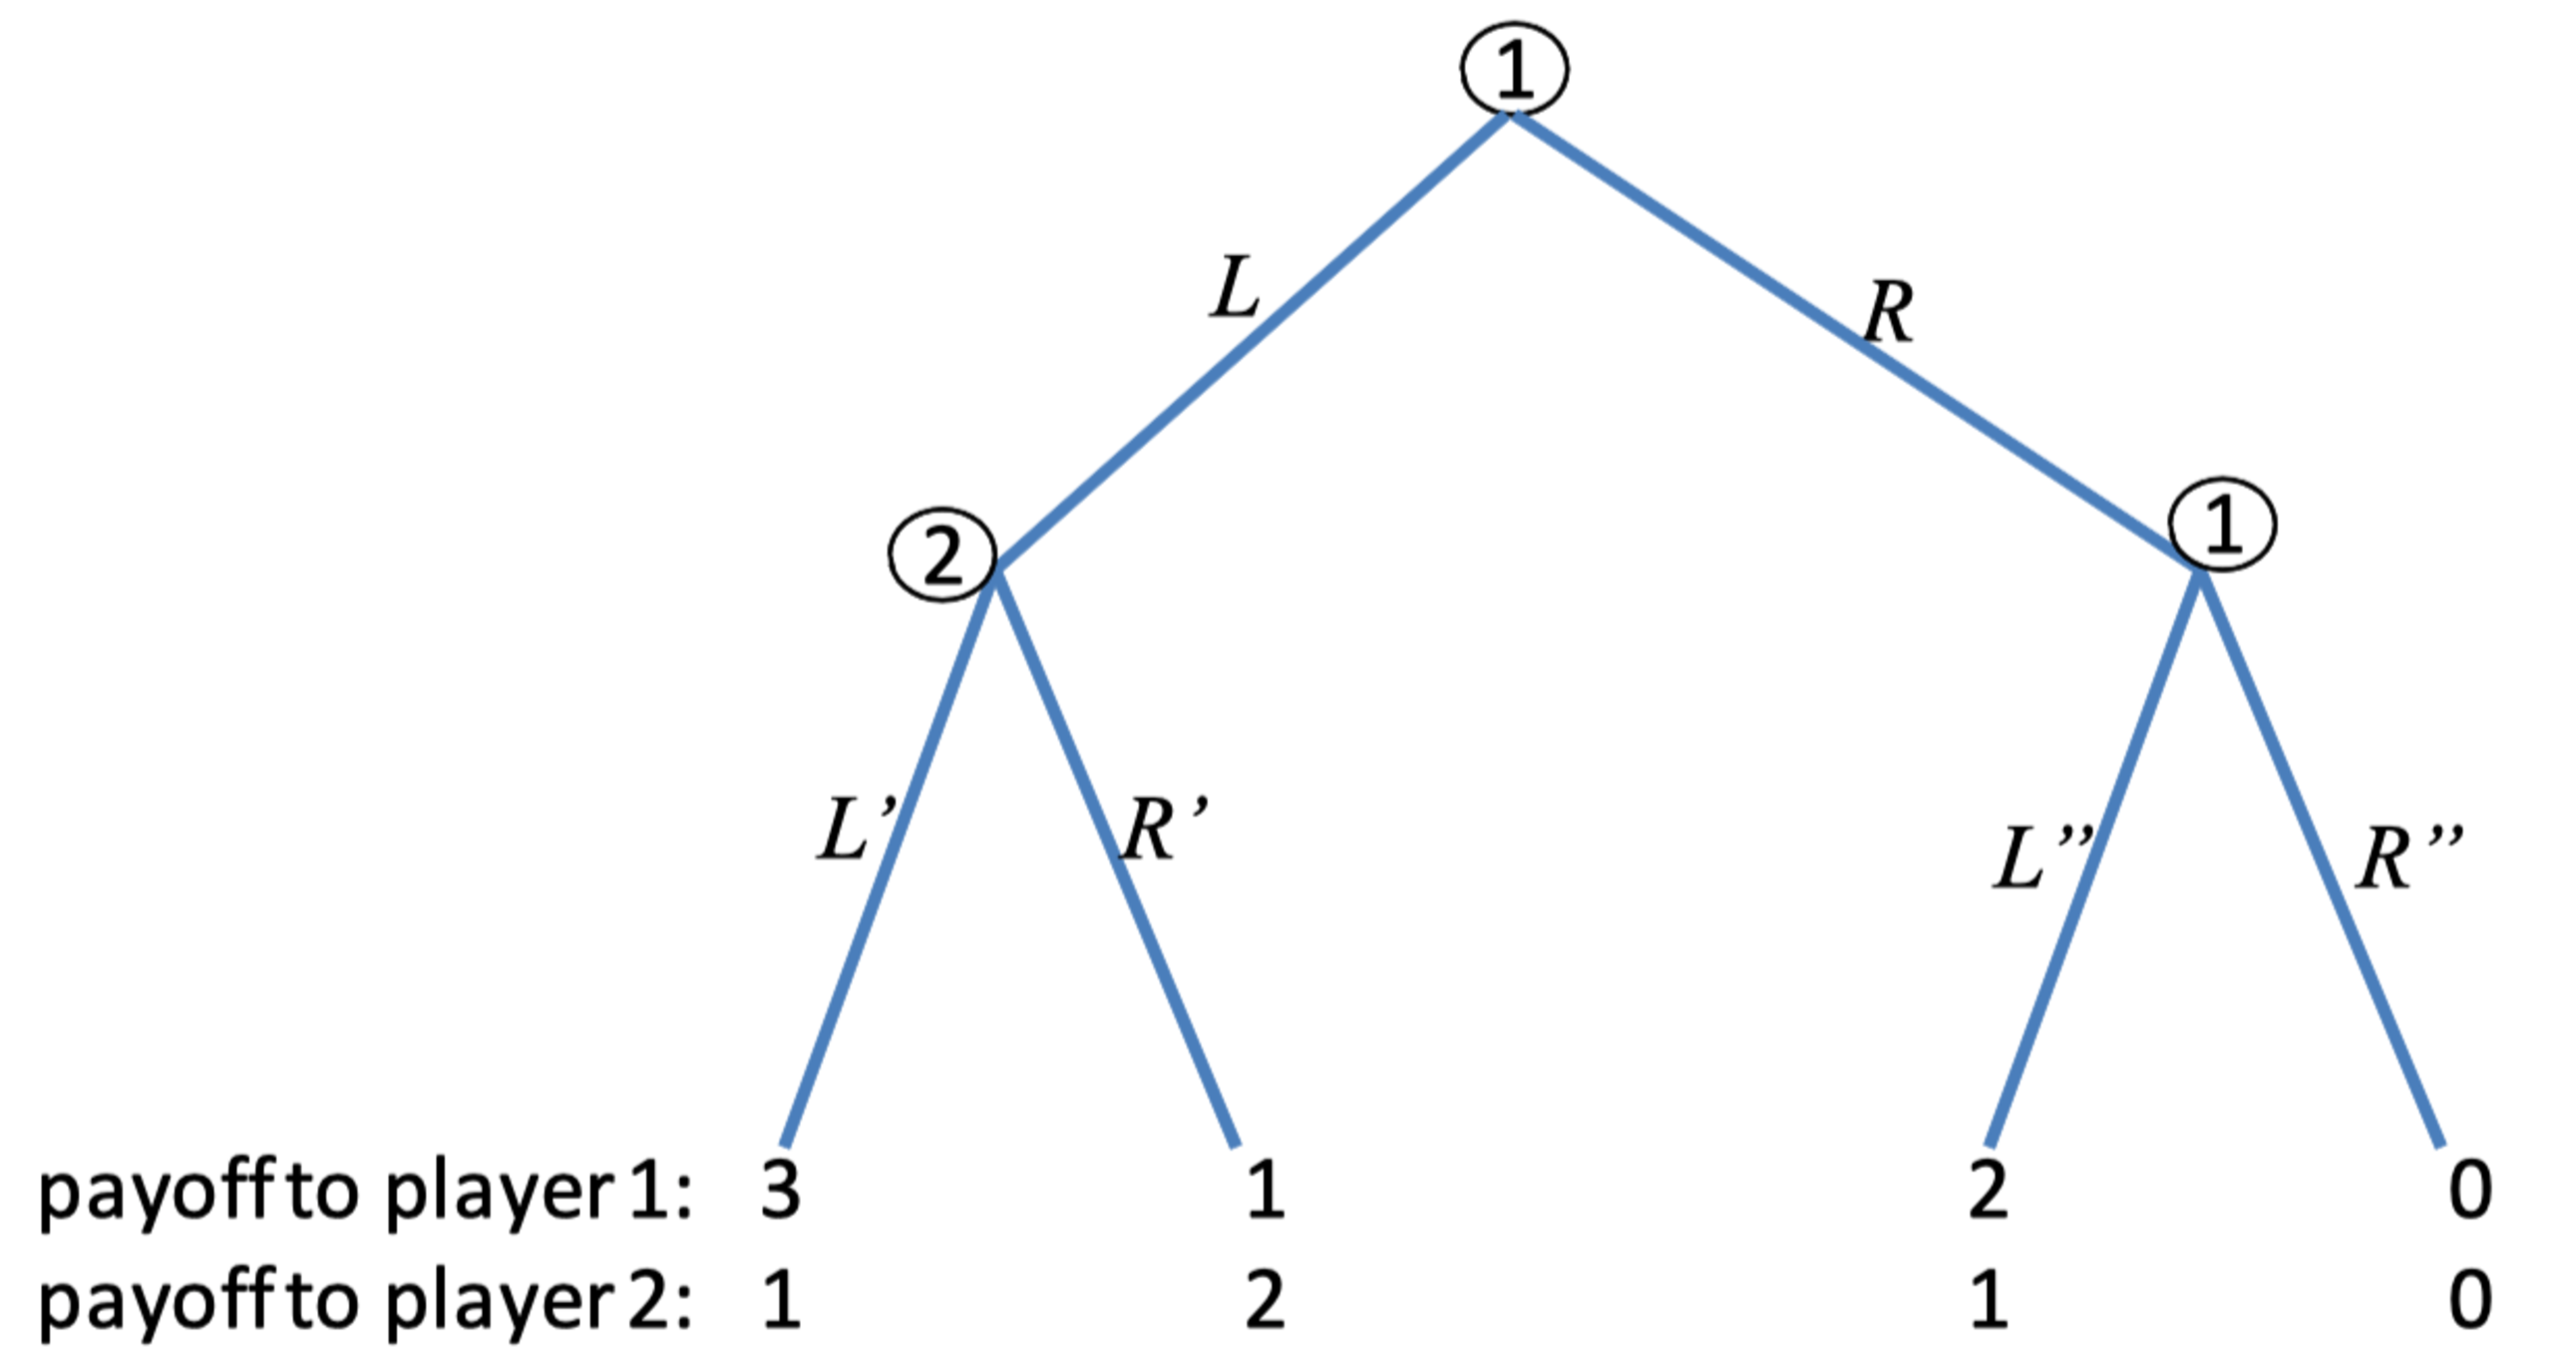
\includegraphics[width=7cm, height=4cm]{game_tree}\par}

\subsubsection{Subgame in extensive-form}
	\begin{tabulary}{\linewidth}{lL}
	1. & begins at a decision node $n$ that is a singleton information set (but not first decision node)\\
	2. & includes all decision and terminal nodes following $n$ in the game tree\\
	3. & does not cut any information sets
	\end{tabulary}

\subsection{1. Set up: Strategy}

\subsubsection{Strategy}
	Complete plan of actions, specifies feasible actions for each player in every contingency (or information set)\\
	$f$(contingency1, contingency2) $\rightarrow$ (action1, action2)

\subsubsection{Mixed Strategies}
	mixed strategy for player $i$ is a probability distribution $p_i=\{p_{ik}\}~\forall k\in[1,K]$ for corresponding $S_i=\{s_{ik}\}$\\
	$0\leq p_{ik}\leq 1$ and $\sum^K_1 p_ik = 1$

\subsection{1. Set up: Payoff}

\subsubsection{Payoff}
	$u_i(s_i, s_{-i})$

\subsubsection{Expected payoffs}
	$v_i(p_i,p_{-i})=\sum^{J}_{j=1}\sum^{K}_{k=1}\left[p_{1j}p_{2k} u_i(s_{1j}, s_{2k})\right]$

\subsection{2. Simplify}

\subsubsection{Iterated Elimination of Strictly Dominated Strategies}
	$IESD$ eliminate dominated strategies by \textbf{pure} or \textbf{mixed strategy}\\
	$NE$ always survive $IESD$ and unique strategy from $IESD \rightarrow NE$\\
	

\subsection{4. Solution: Equilibrium}

\subsubsection{Nash Equilibrium (Pure strategy)}
	$s_i^*$ is player $i$'s best response to strategies specified for other players
	\begin{align*}
		u_i(s^*_i, s^*_{-i})\geq u_i(s_i, s^*_{-i})\Leftrightarrow max_{s_i \in S_i} u_i(s_i, s_{-i}^*)
	\end{align*}
	$NE$ can exist as a set of values $e.g. \{s^*\mid s_1^*+s_2^*=1\}\cup\{(1,1)\}$

\subsubsection{Nash Equilibrium (Mixed Strategies)}
	$p_i^*$ is player $i$'s best response to strategies specified for other players
	\begin{align*}
		v_i(p^*_i, p^*_{-i})\geq v_i(p_i, p^*_{-i})\Leftrightarrow max_{p_i \in P_i} v_i(p_i, p_{-i}^*)
	\end{align*}

\subsubsection{Backward-Induction Outcome}
	every finite game with perfect information has an SPNE, which can be found by backwards induction
	\begin{enumerate}
		\item start with last players: each of last players choose strategy maximising their payoffs
		\item now with second last players: take last players' strategy as given then select their strategy
		\item continue until the beginning of game
	\end{enumerate}
	The BI outcome is $(a_1^*, R_2(a^*_1))$ but subgame perfect NE is $(a^*_1, R_2(a_1))$

\subsubsection{Subgame-Perfect Nash Equilibrium}
	A Nash equilibrium is subgame-perfect if the players' strategies constitute a Nash equilibrium in every (proper) subgame\\
	Subgame perfect outcome is $(a^*_1, a^*_2, a^*_3(a^*_1, a^*_2), a^*_4(a^*_1, a^*_2))$ but subgame perfect NE is $(a^*_1, a^*_2, a^*_3(a_1, a_2), a^*_4(a_1, a_2))$

\section{Solving Static Games of Complete Information with Pure Strategy}
	first form normal-form game, then solve by
	\begin{enumerate}
		\item maximisation problem\\
		$max_{p_i \in P_i} u_i(p_i, p_{-i}^*) \Rightarrow \frac{d}{d p_i}=0$ then solve $n$ players' optimal strategies simultaneously 
		\item graphically\\
		plot $S_i$ against $S_j$ to find intersection
		\item $IESD$\\
		eliminate the impossible strategies by taking the first step in game, then repeat till equilibrium is reached
	\end{enumerate}






% common games

\subsection{Splitting a pie}
	2 players choose to split a dollar $S_i = [0,1]$\\
	$NE$: $\{s^*|s^*_1+s^*_2=1, s^*_1,s^*_2\geq 0\}\cup\{(1,1)\}$
	\begin{align*}
		u_i(s_i, s_{-i}) &=
		\begin{cases}
			s_i, 		&	s_1 + s_2 \leq 1\\
			0, 		&	s_1+s_2 >1
		\end{cases}\\
		R_i(s_{-i}) &= 
		\begin{cases}
			1-s_{-i}, 	&	s_2 < 1\\
			[0,1], 	&	s_{-i} = 1
		\end{cases}
	\end{align*}
	{\centering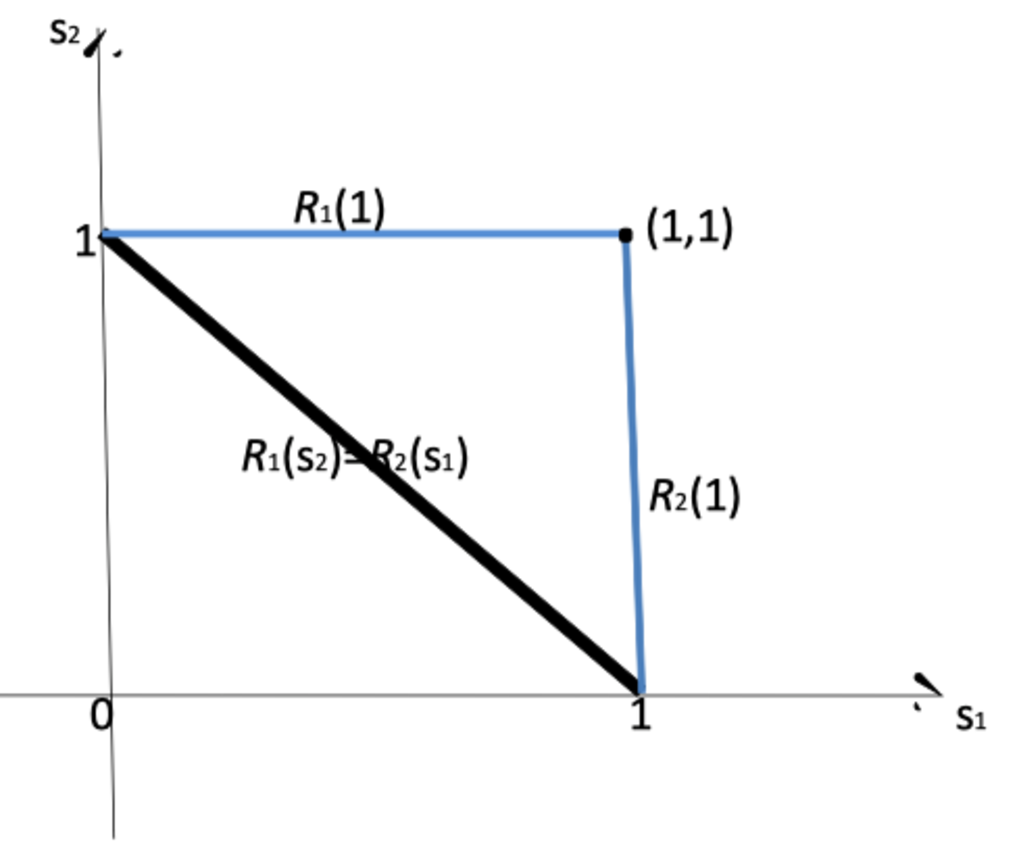
\includegraphics[width=4cm, height=4cm]{splitting_coin}\par}

\subsection{Cournot Model of Duopoly}
	2 firms choose \textbf{quantity}, $S_i = [0,\infty), q_i\geq 0$\\
	$NE: (q_1^*,q_2^*)=(\frac{a-c}{3},\frac{a-c}{3})$
	\begin{align*}
		u_i(s_1, s_2): \pi_i(q_1, q_2) &= q_i[a-(q_1+q_2)-c]\\
		R_i(q_j): q_i &= \frac{1}{2}(a-c-q_j)
	\end{align*}
	{\centering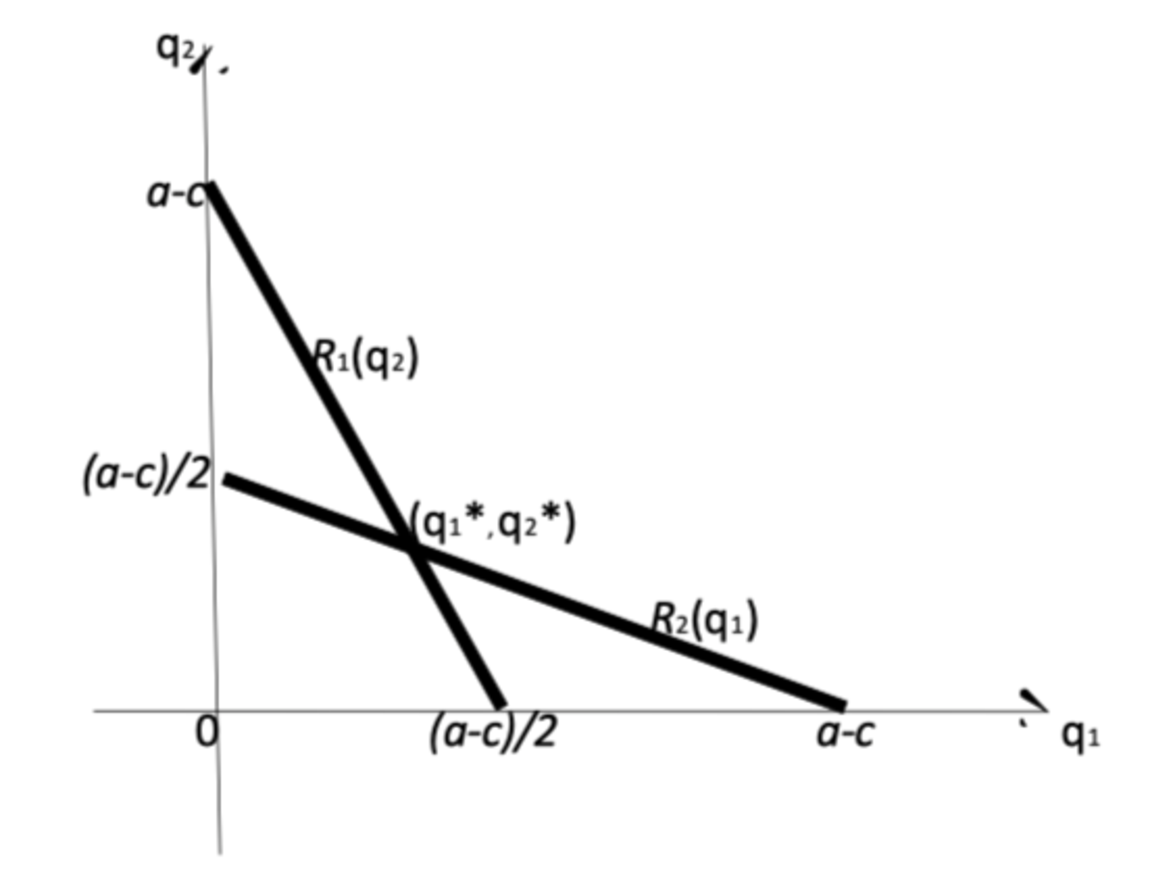
\includegraphics[width=4cm, height=4cm]{cournot}\par}

\subsection{Bertrand Model of Duopoly}
	2 firms choose \textbf{price}, $S_i = [0,\infty), p_i\geq0$\\
	$NE: (p_1^*, p_2^*)=(\frac{a+c}{2-b}, \frac{2+c}{2-b})$
	\begin{align*}
		u_i(s_1,s_2):\pi_i(p_1,p_2)&=(a-p_i+bp_j)(p_i-c)\\
		R_i(p_j) : p_i &= \frac{1}{2}(a+bp_j+c)
	\end{align*}
	$b>0$ for substitute products and marginal cost $c: 0<c<a$\\

\columnbreak
\subsection{Voting (2 players)}
	NE: $(s_1, s_2) = (\frac{1}{2}, \frac{1}{2})$\\
	Player 1, 2 decide of a location on line $s_i \in [0,1]$\\
	\begin{align*}
		u_i(s_i, s_{-i}) = 
		\begin{cases}
			\frac{s_1+s_2}{2}, 	&	s_i \leq s_j\\
			1-\frac{s_1+s_2}{2}, 	&	s_j \leq s_i\\
		\end{cases}
	\end{align*}
	if both players do not choose the same platform, assume $s_i < s_j$, then $i$ can improve payoff by choosing $s_i + \epsilon$\\
	if both players do not choose 0.5 platform, assume they choose $x>0.5$, then each can improve payoff by choosing $s_i - \epsilon$\\
	Note: for 3 players voting there is no pure strategy NE

\subsection{Final-Offer Arbitration}
	Firm offer $w_f$ and Union offer $w_u$, arbitrator with ideal $x$ wage
	\begin{align*}
		w &= 
		\begin{cases}
			w_f,		&	x < (w_f + w_u)/2\\
			w_u,		&	x > (w_f + w_u)/2
		\end{cases}\\
		E(w) &= P(w=w_f)w_f + P(w=w_u)w_u\\
			&= F_X(w_f + w_u)/2)w_f + \left[1-F_X(w_f + w_u)/2)\right]w_u
	\end{align*}
	solving for $\max_{w_f}E(w)$ and $\max_{w_u}E(w)$\\
	$\Rightarrow (w_u^* - w_f^*)\cdot \frac{1}{2}f_X(\frac{w^*_f+w^*_u}{2}) = F(\frac{w^*_f+w^*_u}{2}) = 1- F(\frac{w^*_f+w^*_u}{2})$\\
	$\Rightarrow F(\frac{w^*_f+w^*_u}{2}) = \frac{1}{2}$ and $w_u^*-w_f^* = \frac{1}{f_X(\frac{w^*_f+w^*_u}{2})}$\\
	Assume $x\sim N(m, \sigma^2)$, from $F(\frac{w^*_f+w^*_u}{2}) = \frac{1}{2} \Rightarrow \frac{w^*_f+w^*_u}{2} = m$\\
	$w_u^*-w_f^* = \frac{1}{f_X(\frac{w^*_f+w^*_u}{2})} = \sqrt{2\pi\sigma^2}$\\
	Solving the two equations, NE: $(w^*_u, w^*_f) = (m+\sqrt{\frac{\pi\sigma^2}{2}}, m-\sqrt{\frac{\pi\sigma^2}{2}})$
	
\subsection{The Problems of the Commons}
	farms $i \in [1, n]$ keeps goat $g_i$, $G = \sum g_i$, grazing benefit $v(G)$
	\begin{align*}
		u_i = g_iv(G) - cg_i
	\end{align*}\\
	$\max_{g_i} u_i \Rightarrow g_iv'(G) + v(G) - c =0 =  \frac{1}{n}G^*v'(G^*) + v(G^*) - c$\\
	but for society: $\max_G u \Rightarrow G^{**}v'(G^{**}) + v(G^{**}) - c$\\
	since $G^* > G^{**}$, common resource is overutilised

\section{Solving Static Games of Complete Information with Mixed Strategy}

\subsection{Matching Pennies}
	{\centering\begin{tabular}{r|cc}
				&	heads	&	tails\\
		\hline
		heads	&	-1,1		&	1,-1\\
		tails		&	1,-1		&	-1,1
	\end{tabular}\par}
	MSNE: $(p_1^*, p_2^*) = (\frac{1}{2}H+\frac{1}{2}T, \frac{1}{2}H+\frac{1}{2}T)$\\
	$p_1 = (r, 1-r), p_2 = (q, 1-q)$
	\begin{align*}
		v_1(p_1, p_2) 	=& r\cdot q\cdot (-1) + (1-r)\cdot q\cdot (1) \\
					+& r\cdot (1-q)\cdot (1) + (1-r)\cdot (1-q)\cdot (-1)\\
				 	=& -4rq + 2r + 2q - 1\\
		R_2(r): q(r) 	=& \frac{1}{2}
	\end{align*}
\subsubsection{graphically}
	\begin{align*}
		v_1(s_{11}, p_2) &= q\cdot(-1) + (1-q)\cdot 1 = 1-2q\\
		v_1(s_{12}, p_2) &= q\cdot 1 + (1-q)\cdot (-1) = -1+2q\\
		r(q) &=
		\begin{cases}
			1, & q<\frac{1}{2}\\
			[0,1], & q=\frac{1}{2}\\
			0, & q > \frac{1}{2}
		\end{cases}
	\end{align*}
	{\centering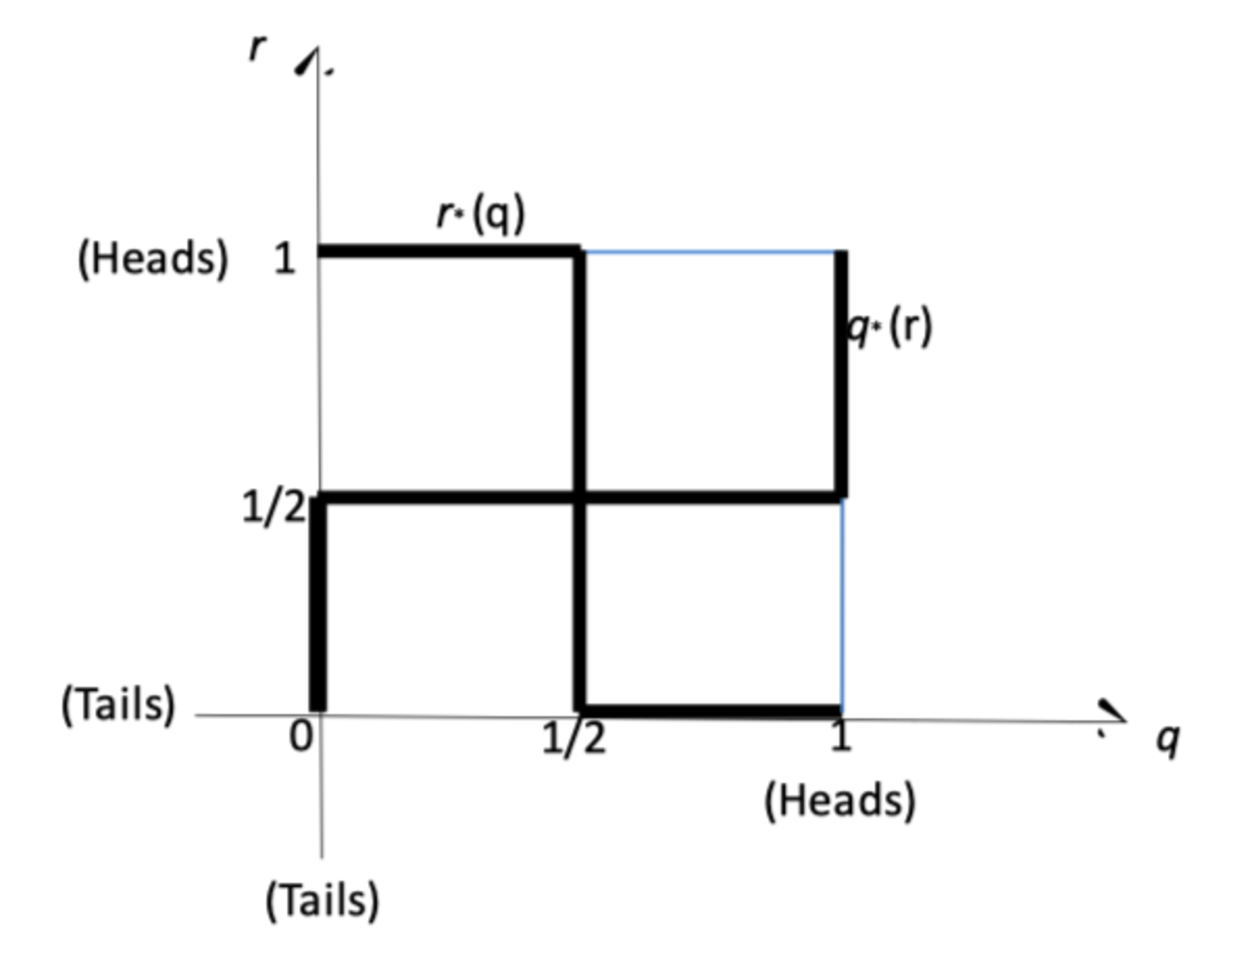
\includegraphics[width=4cm, height=4cm]{matching_pennies}\par}

\section{Solving Dynamic Games of Complete and Perfect Information}
	Besides (player, strategy, payoff), \textbf{timing} is required\\
	Theory: Backwards Induction

\subsection{Entry Deterrence}
	BI outcome: $(E, \bar F)$\\
	{\centering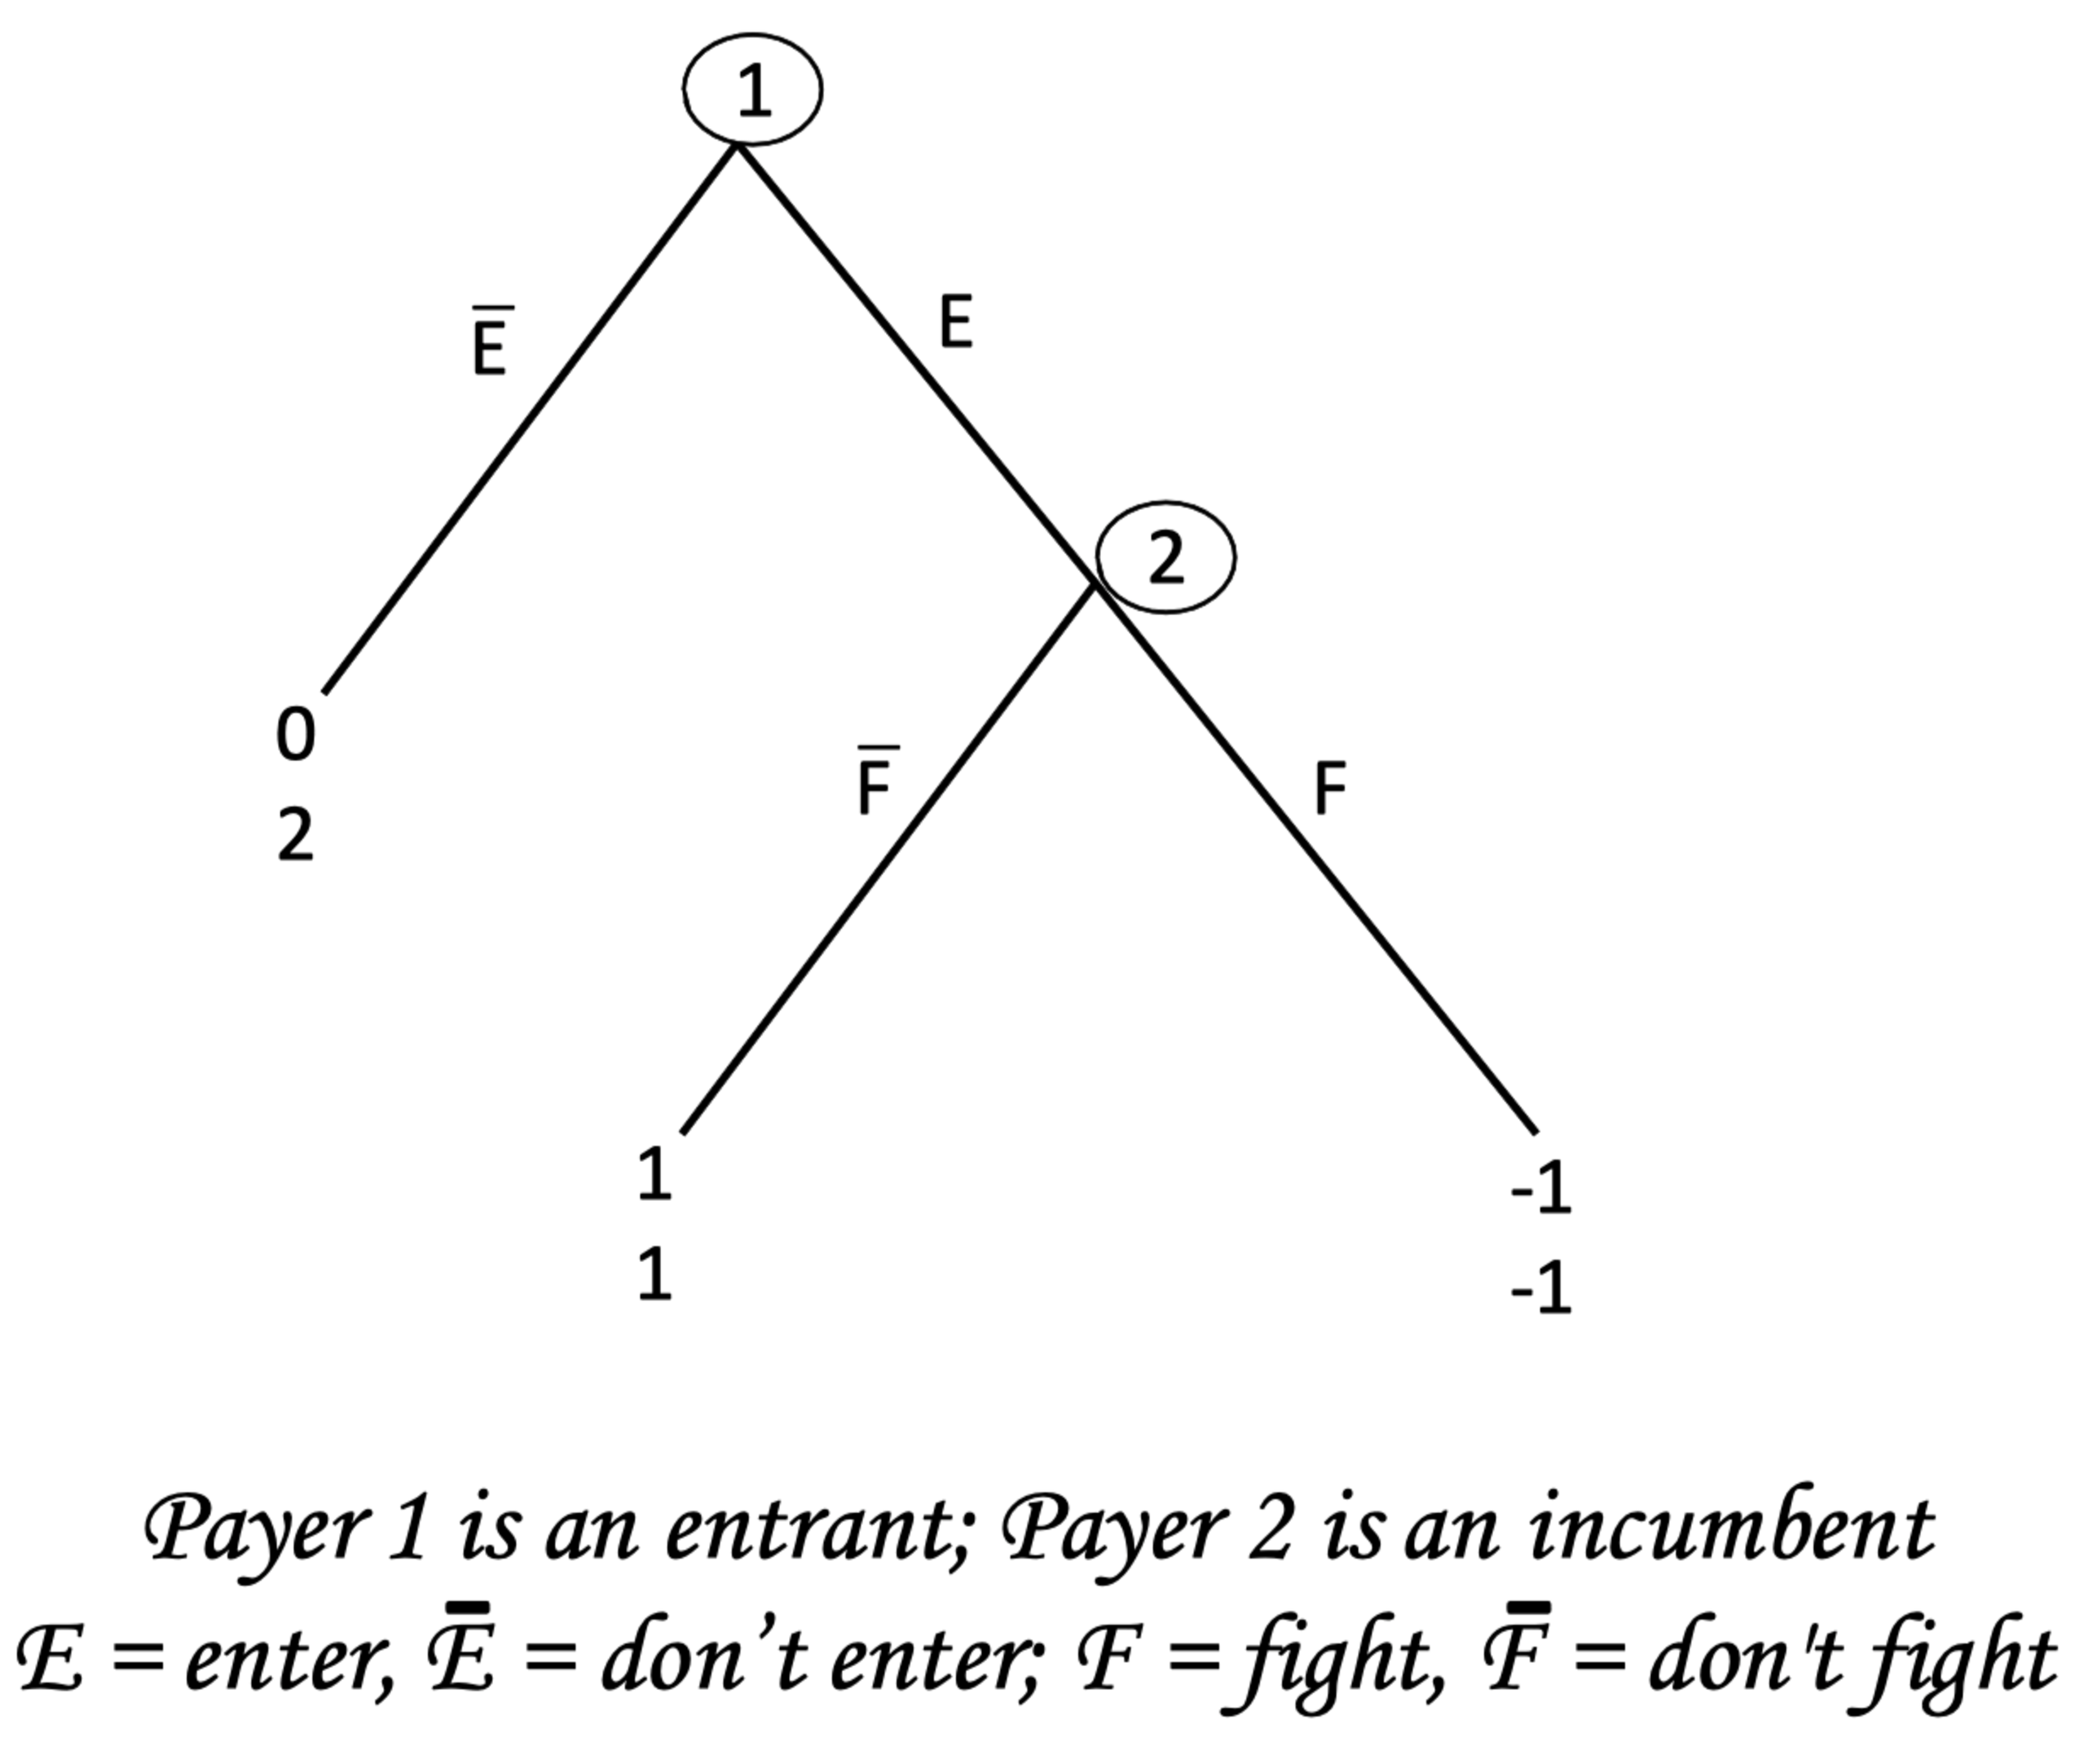
\includegraphics[width=4cm, height=4cm]{entry_deterrence}\par}

\subsection{The Frog and the Scorpion}
	BI outcome: (don't help, sting)\\
	{\centering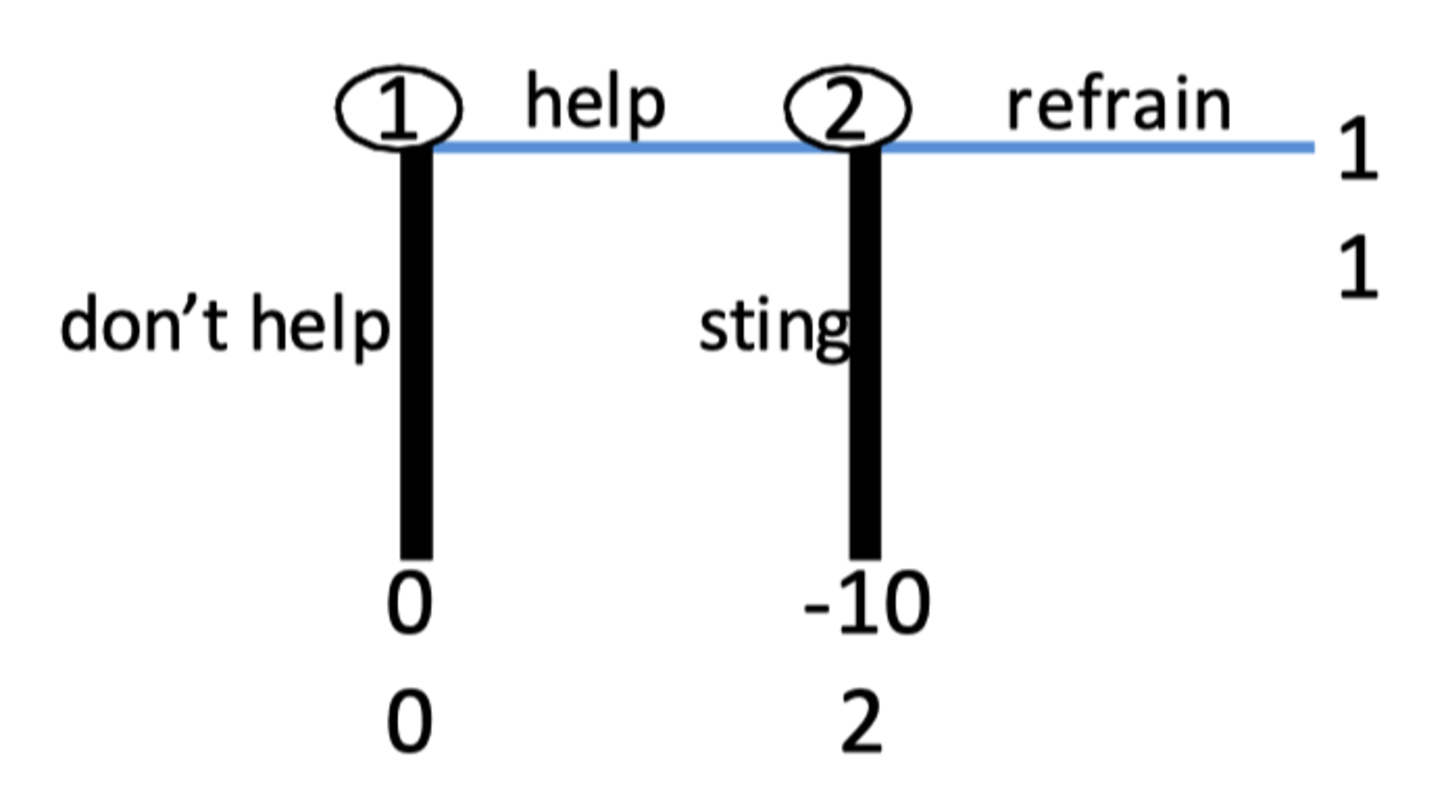
\includegraphics[width=4cm, height=3cm]{frog_scorpion}\par}

\subsection{Centipede game}
	BI outcome: $(s_1, s_2, s_3, s_4, s_5, s_6)$\\
	{\centering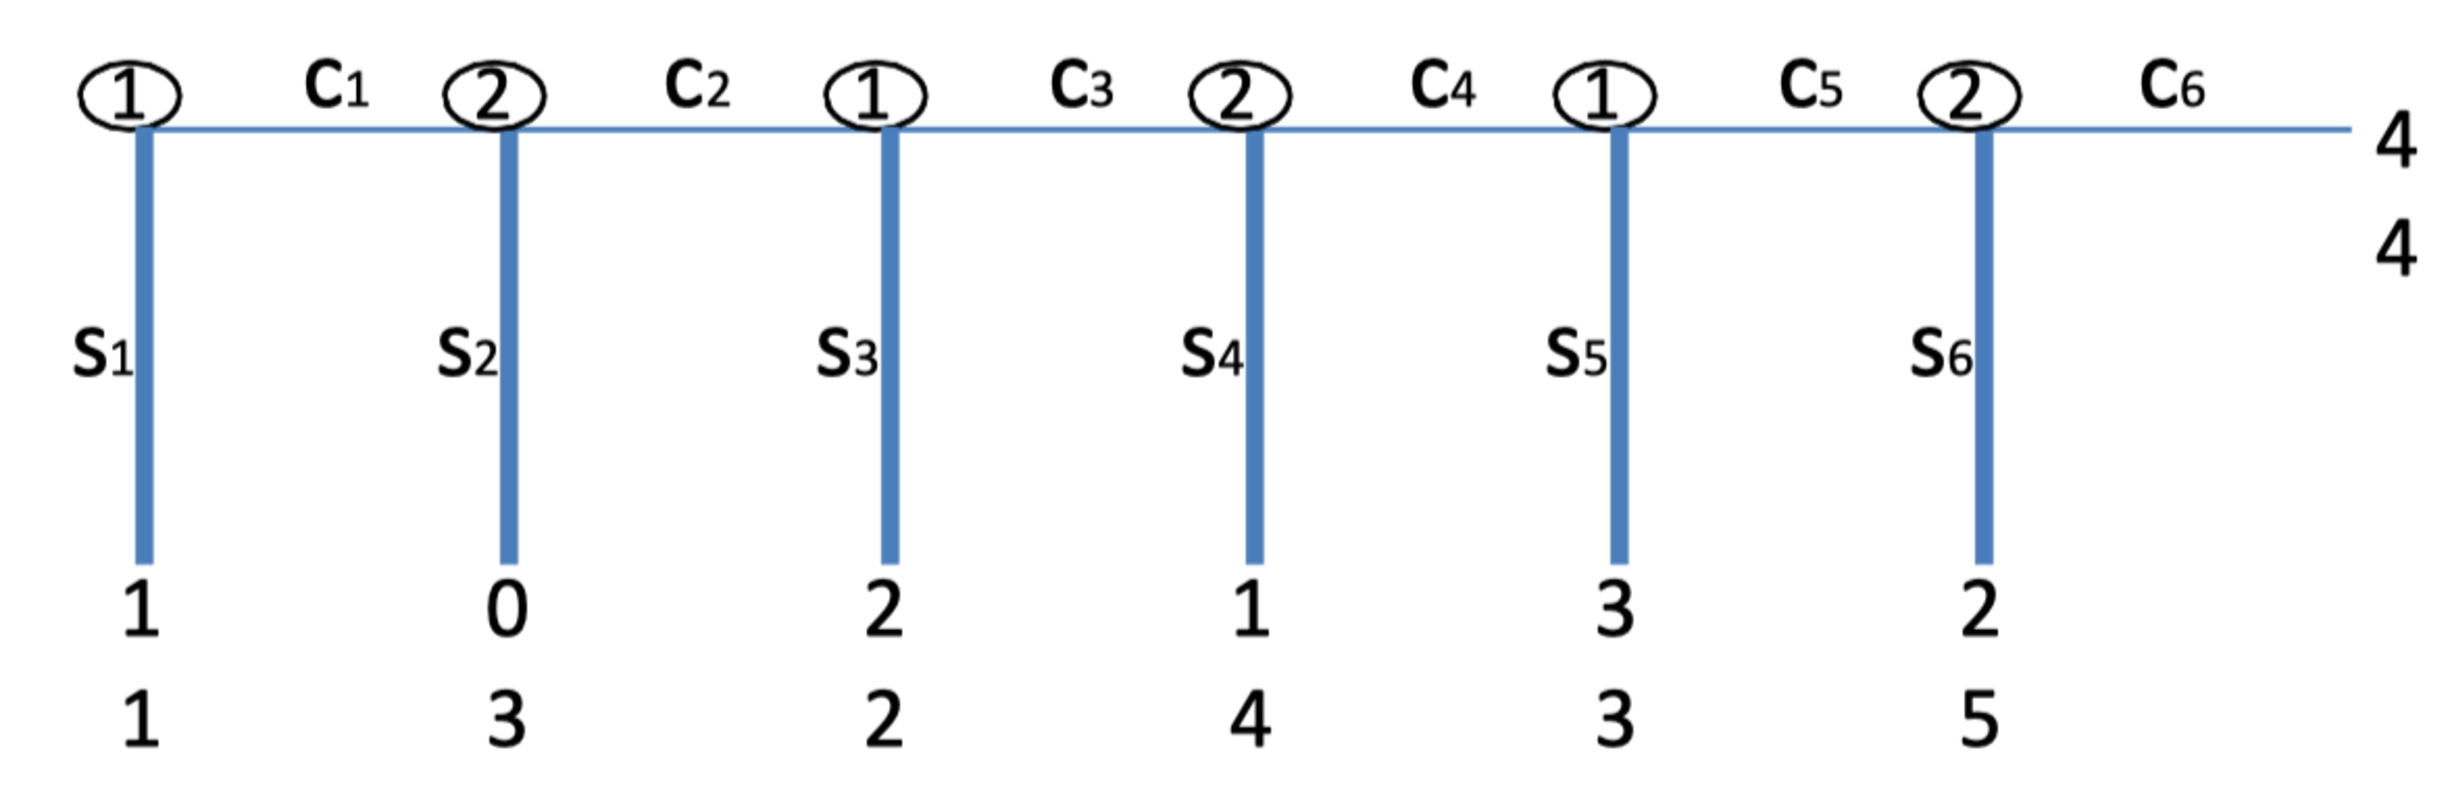
\includegraphics[width=6cm, height=3cm]{centipede}\par}

\subsection{Stackelberg Duopoly}
	a leader and follower deciding on output to produce\\
	timing: \\
	1. leader $q_1\geq 0$\\
	2. follower observe then $q_2\geq 0$\\
	BI outcome: $(q_1^*, q_2^*) = \left( \frac{a-c}{2}, \frac{a-c}{4} \right)$
	\begin{align*}
		u_i: \pi_i(q_i, q_j) &= P(Q)q_i - cq_i\\
		R_2(q_1) &= \frac{1}{2}(a-c-q_1)\\
		\pi_1(q_1, R_2(q_1)) &= \frac{1}{2}(a-c-q_1)q_1\\
		R_1(q_2) &= \frac{a-c}{2}
	\end{align*}
	{\centering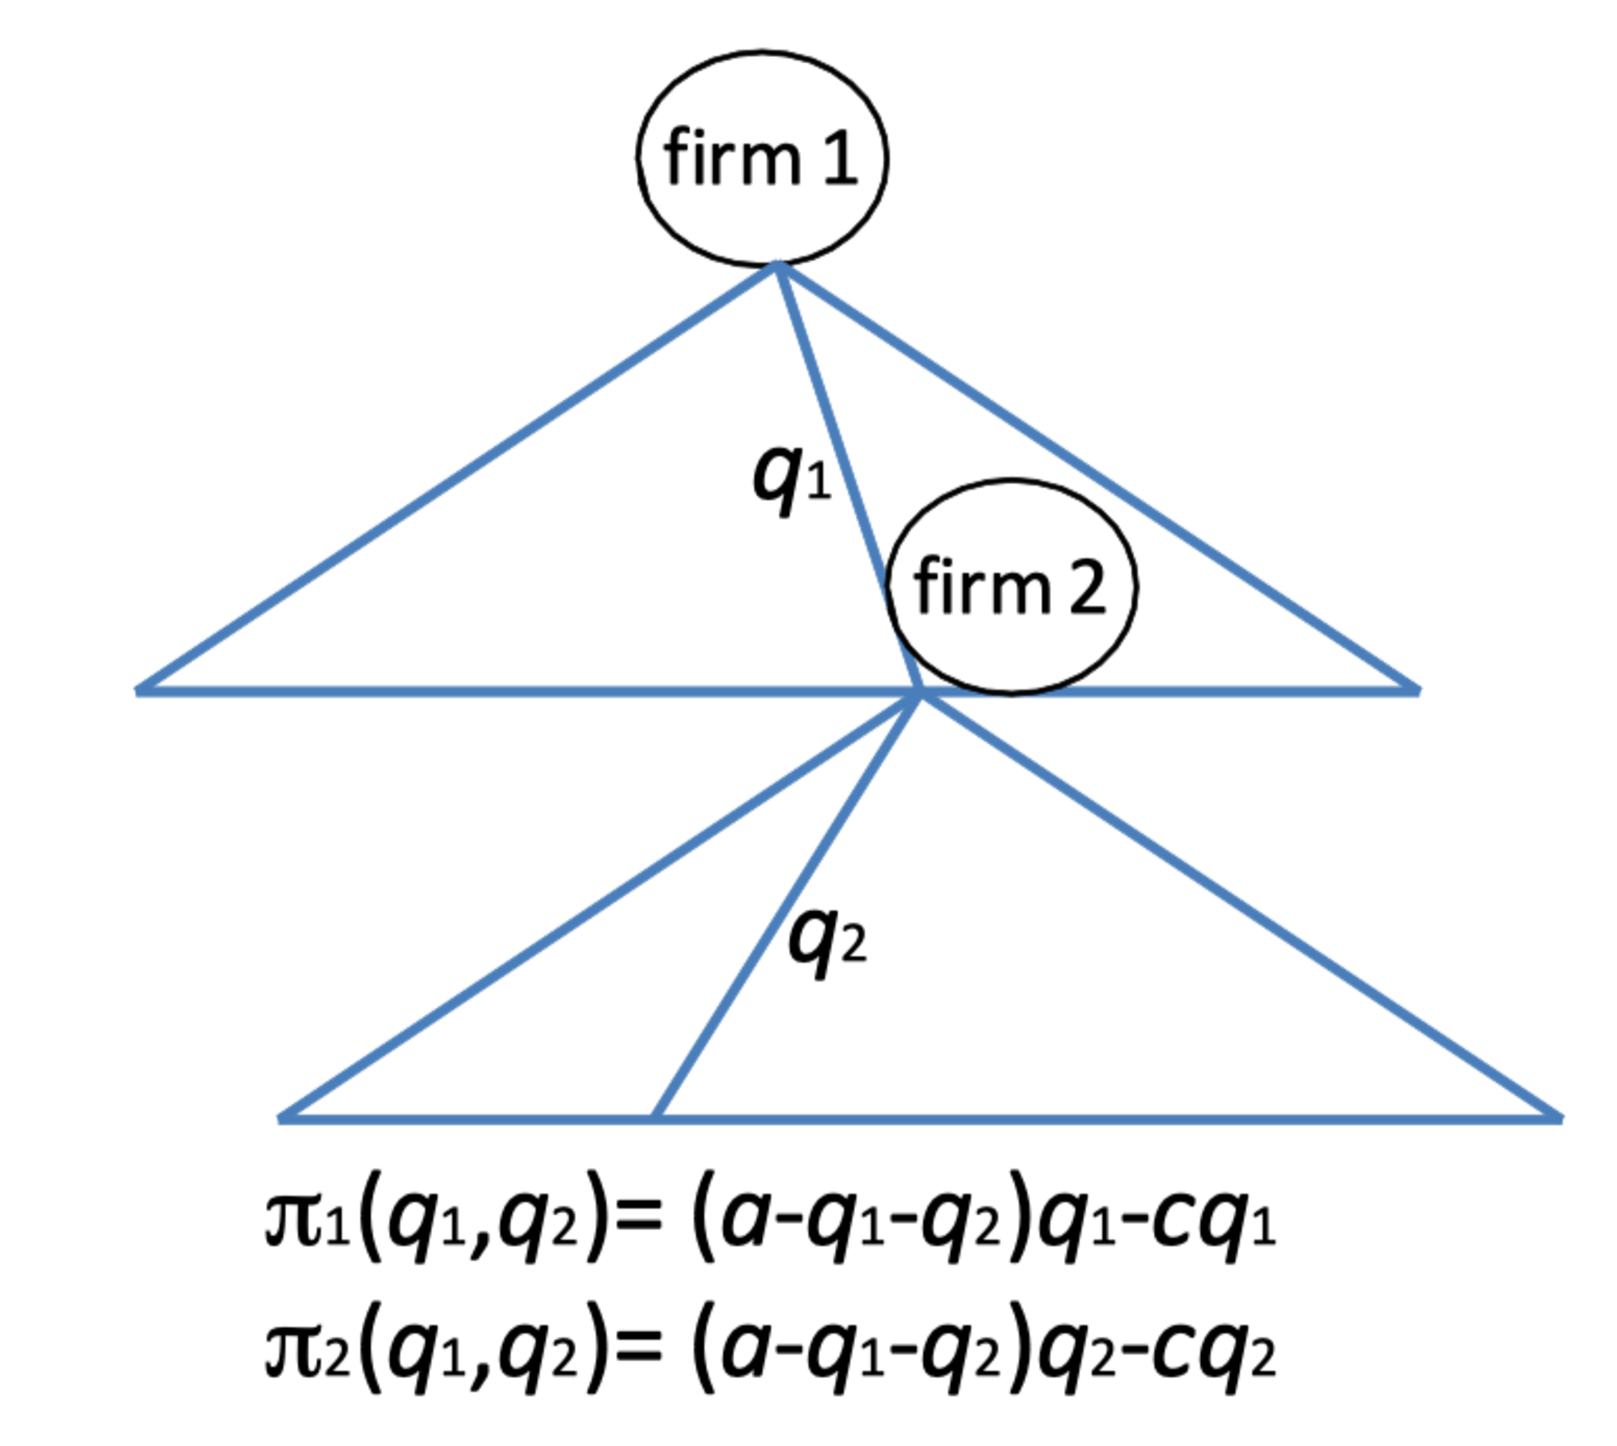
\includegraphics[width=4cm, height=4cm]{stackelberg}\par}

%\subsection{Wages and Employment in a Unionised Firm}
%	yet to play

\columnbreak
\subsection{Sequential Bargaining (1-Period)}
	player 1, 2 splitting pie\\
	timing: \\
	1. player 1 propose $s_1$, leave $1-s_1$ for player 2\\
	2. player 2 then accept/reject\\
	BI outcome: $(s^*_1=1, R_2(s^*_1)$ = accept)\\
	{\centering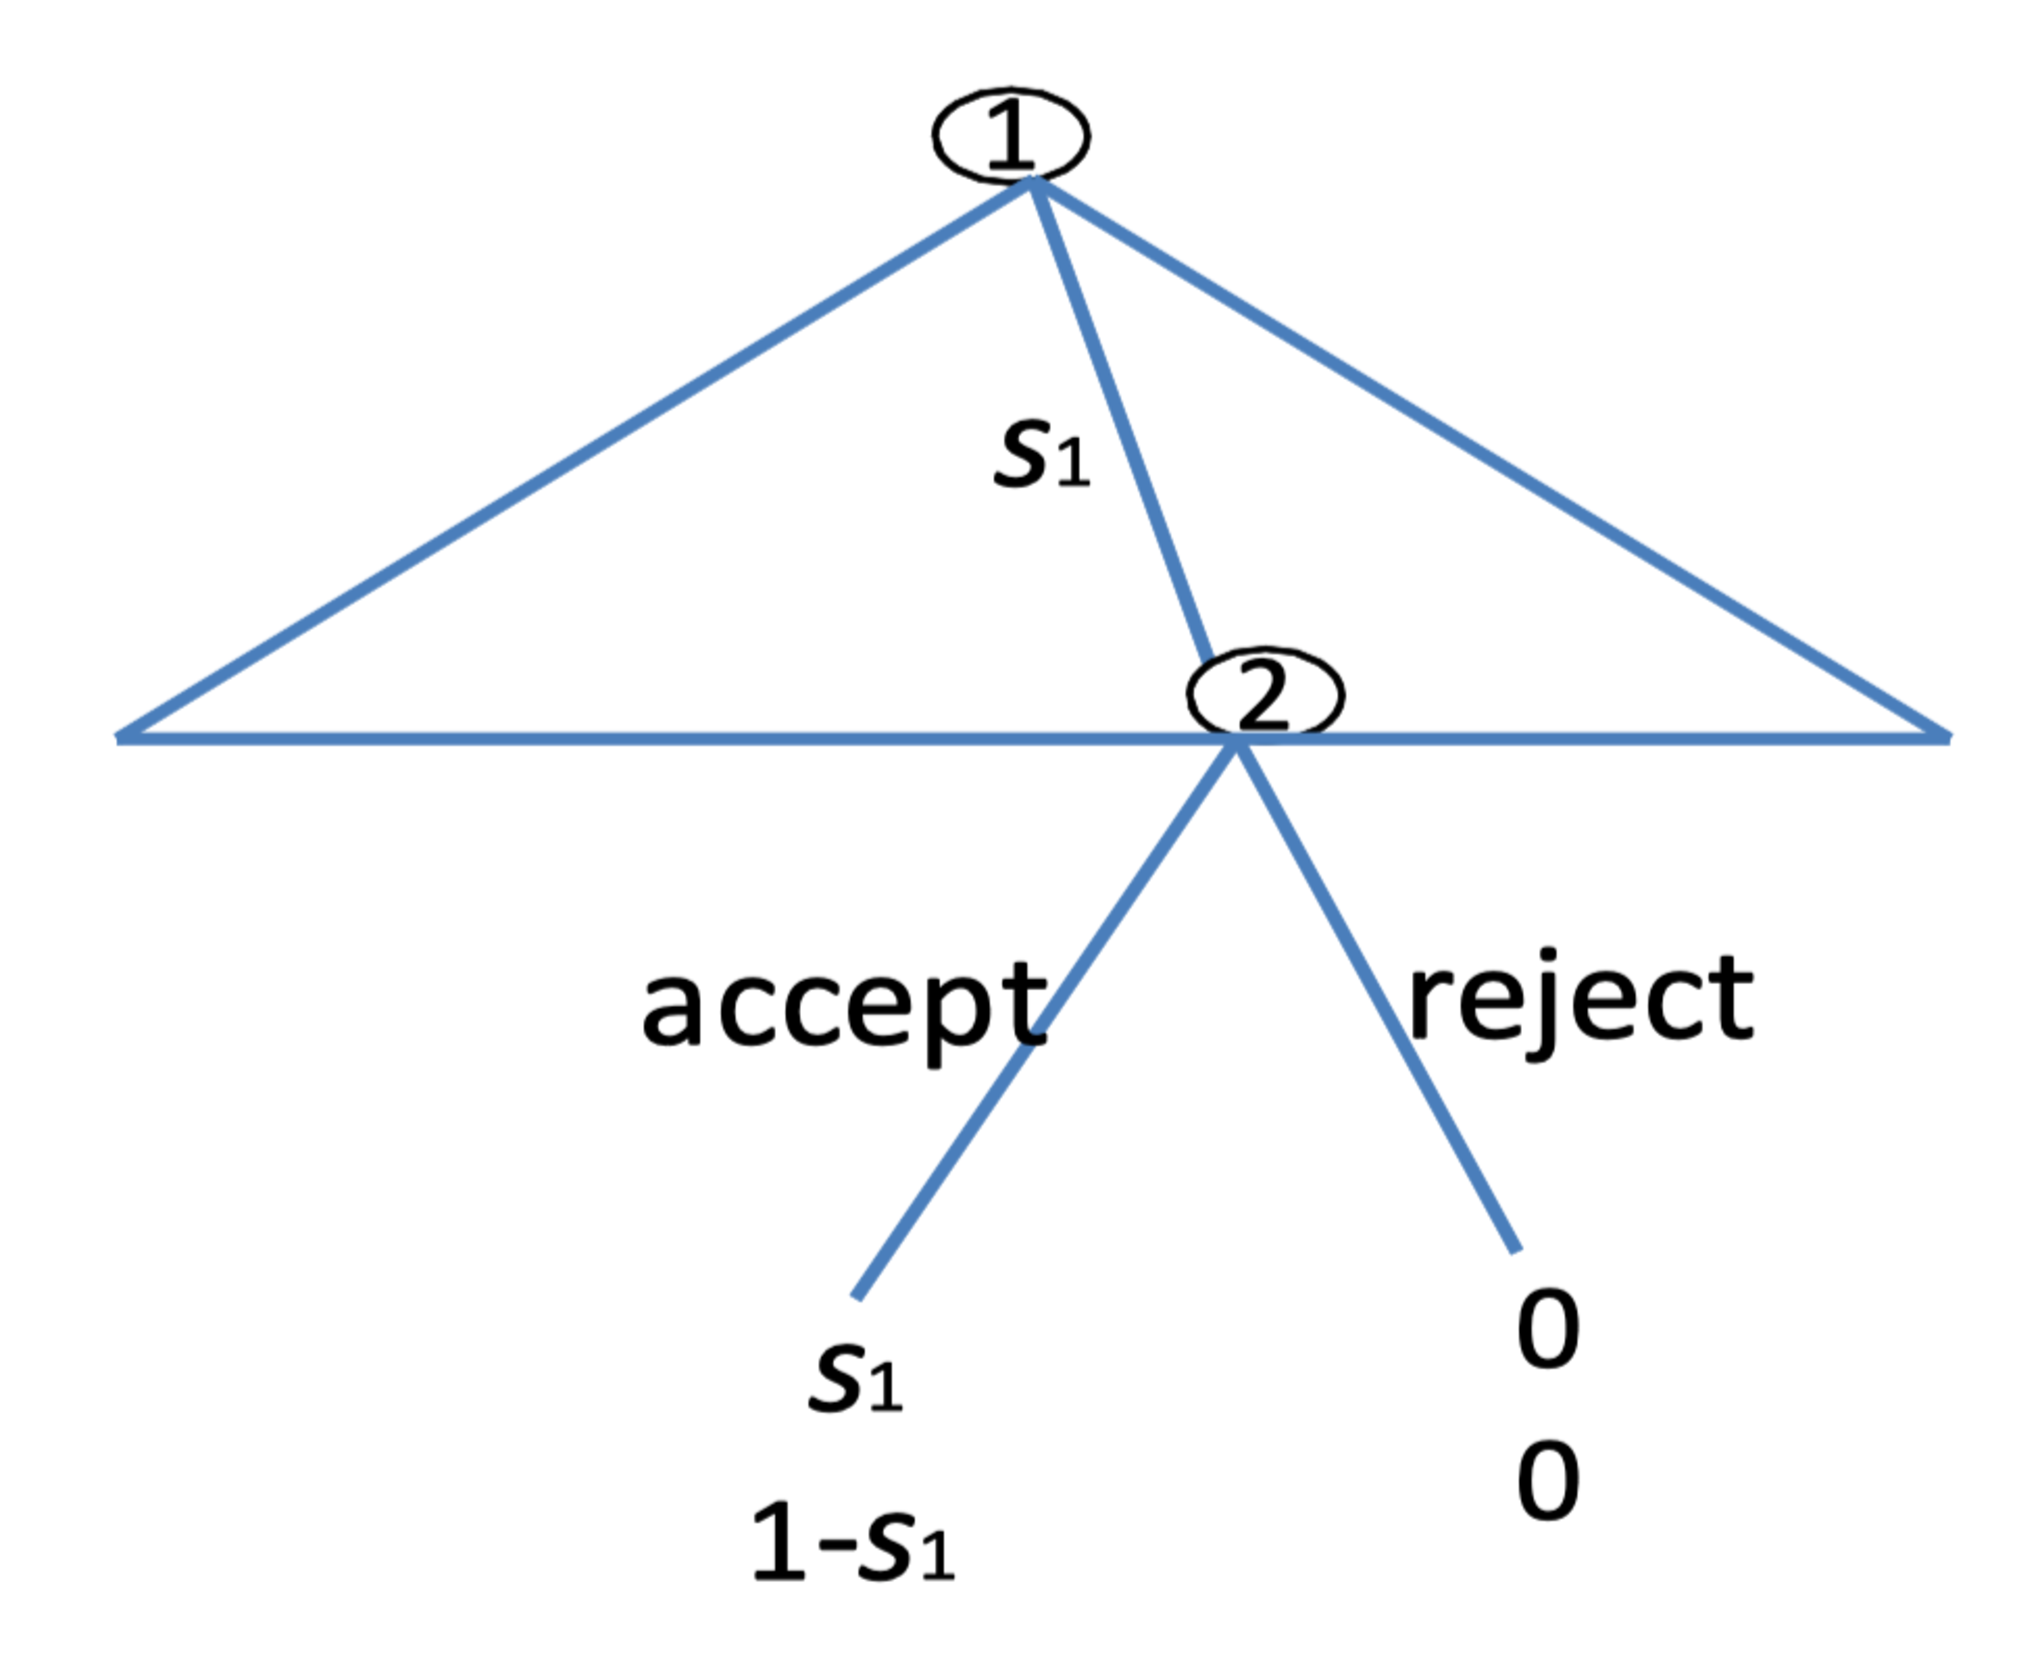
\includegraphics[width=4cm, height=4cm]{bargin_1period}\par}

\subsection{Sequential Bargaining (3-Period)}
	player 1, 2 splitting pie\\
	timing: \\
	1. player 1 propose $s_1$, leave $1-s_1$ for player 2\\
	2. player 2 then accept/reject, if reject then continue\\
	3. game repeat till period 3\\
	BI outcome: 1 offer  $(s^*_1, 1-s^*_1)$ and 2 accept immediately\\
	$(s^*_2, 1-s^*_2) = (\delta s, 1-\delta s)$\\
	player 1 accepts iif $s_2 \geq \delta s$\\
	$(s^*_1, 1-s^*_1) = (1-\delta(1-\delta s), \delta(1-\delta s))$\\
	player 2 accepts iif $1 - s_1 \geq \delta(1-\delta s)$\\
	{\centering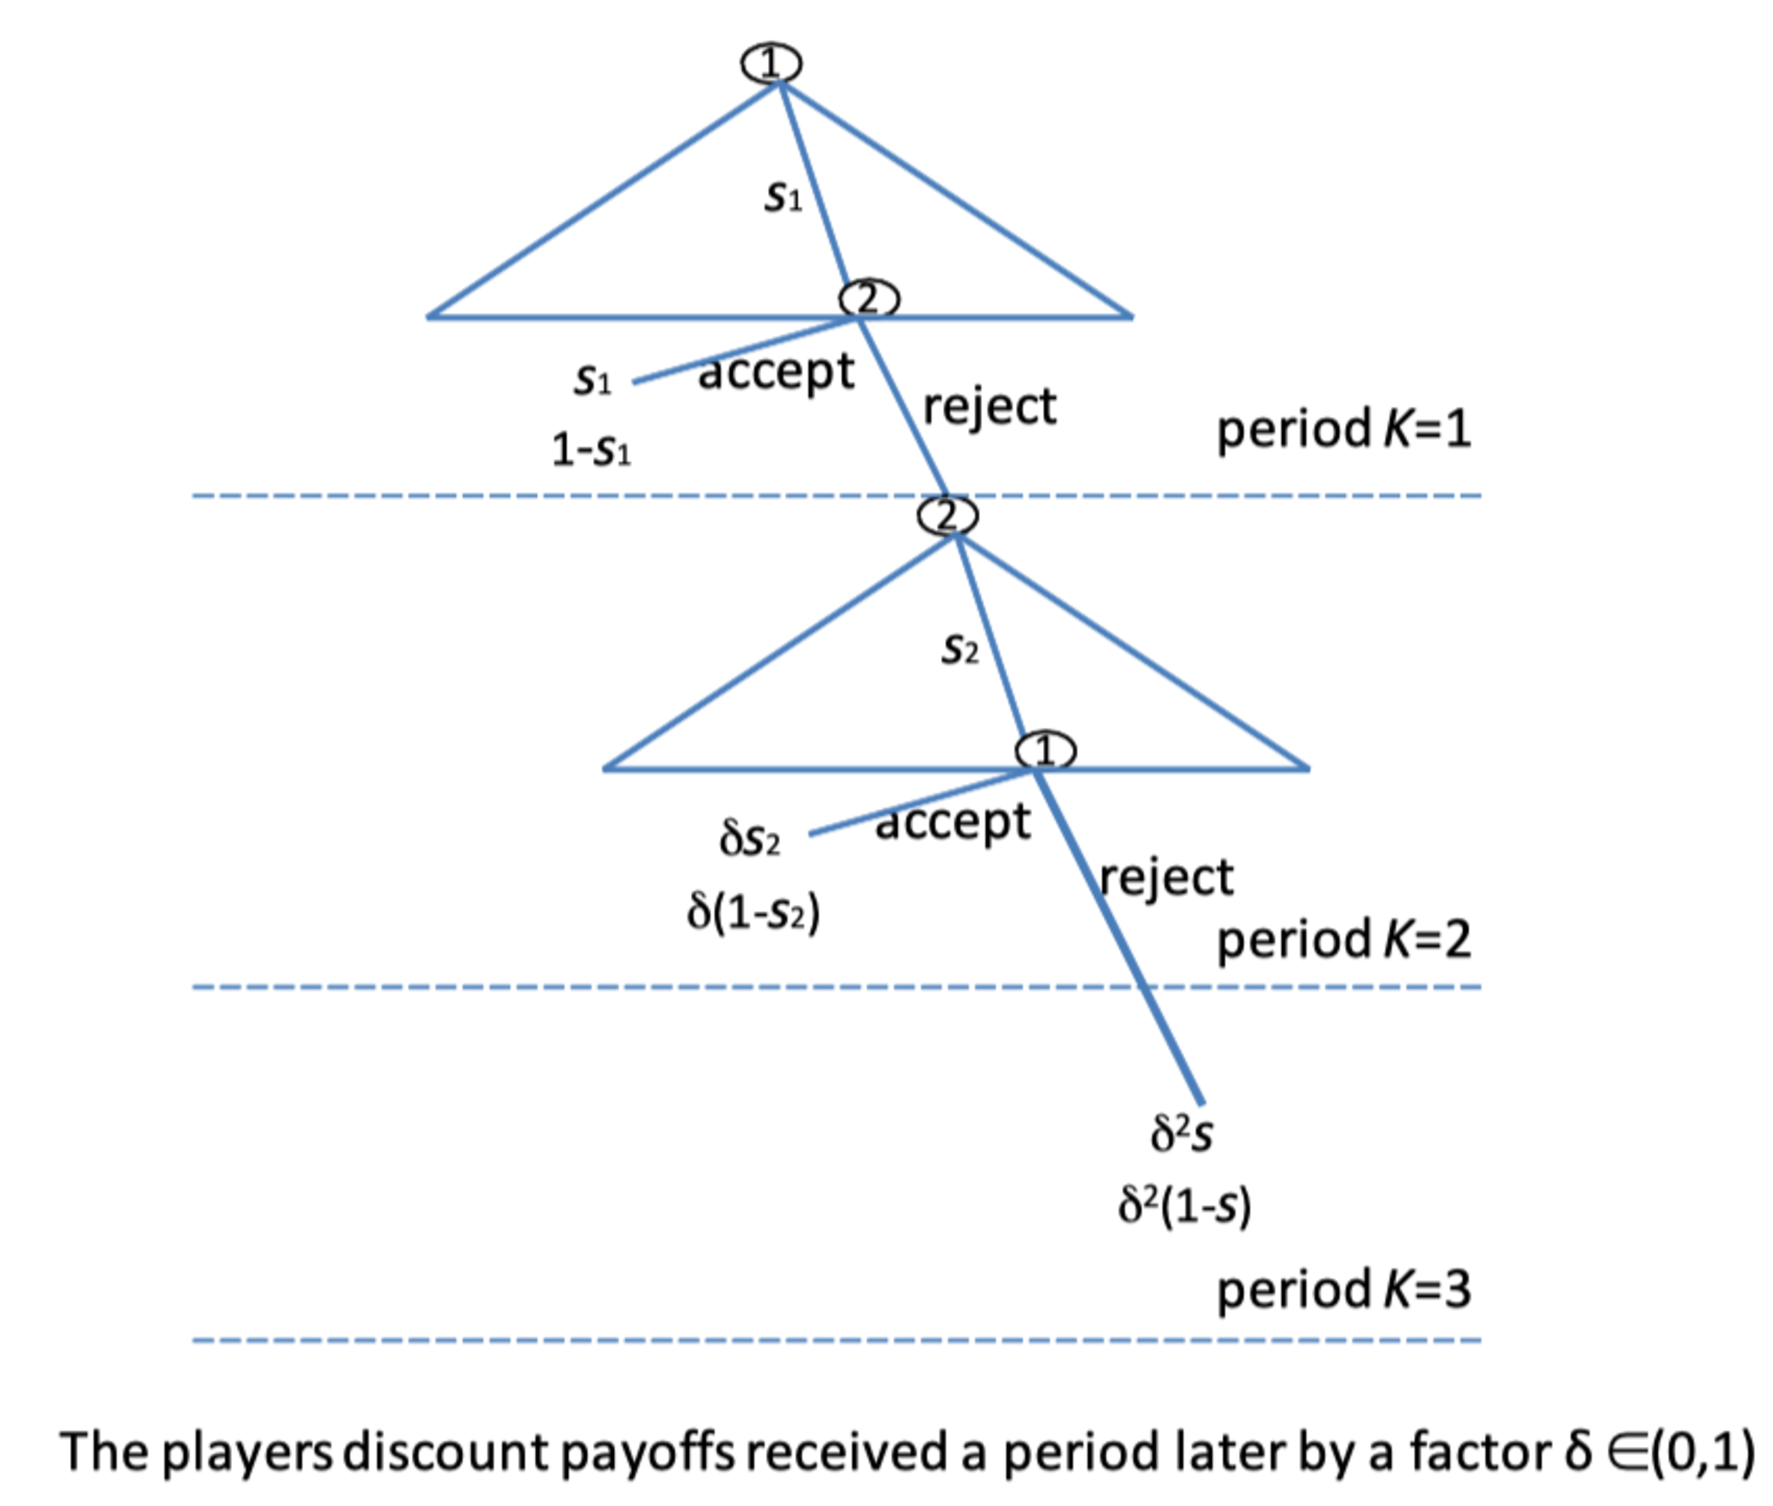
\includegraphics[width=4cm, height=4cm]{bargin_3period}\par}
	Note: they are only comparing between this period and next\\

\columnbreak
\subsection{Rubinstein's Model (Infinite-Period)}
	player 1, 2 splitting pie\\
	timing: \\
	1. player 1 propose $s_1$, leave $1-s_1$ for player 2\\
	2. player 2 then accept/reject, if reject then continue\\
	3. game repeat infinity\\
	BI outcome: player 1 offer $(s^*, 1-s^*) = (\frac{1}{1+\delta}, \frac{\delta}{1+\delta})$\\
	Since when 1 offers $(f(s), 1-f(s))$  2 will accept immediately,
	\begin{align*}
		f(s) = 1-\delta(1-\delta s)
	\end{align*}
	derive answer through G.S.\\
	{\centering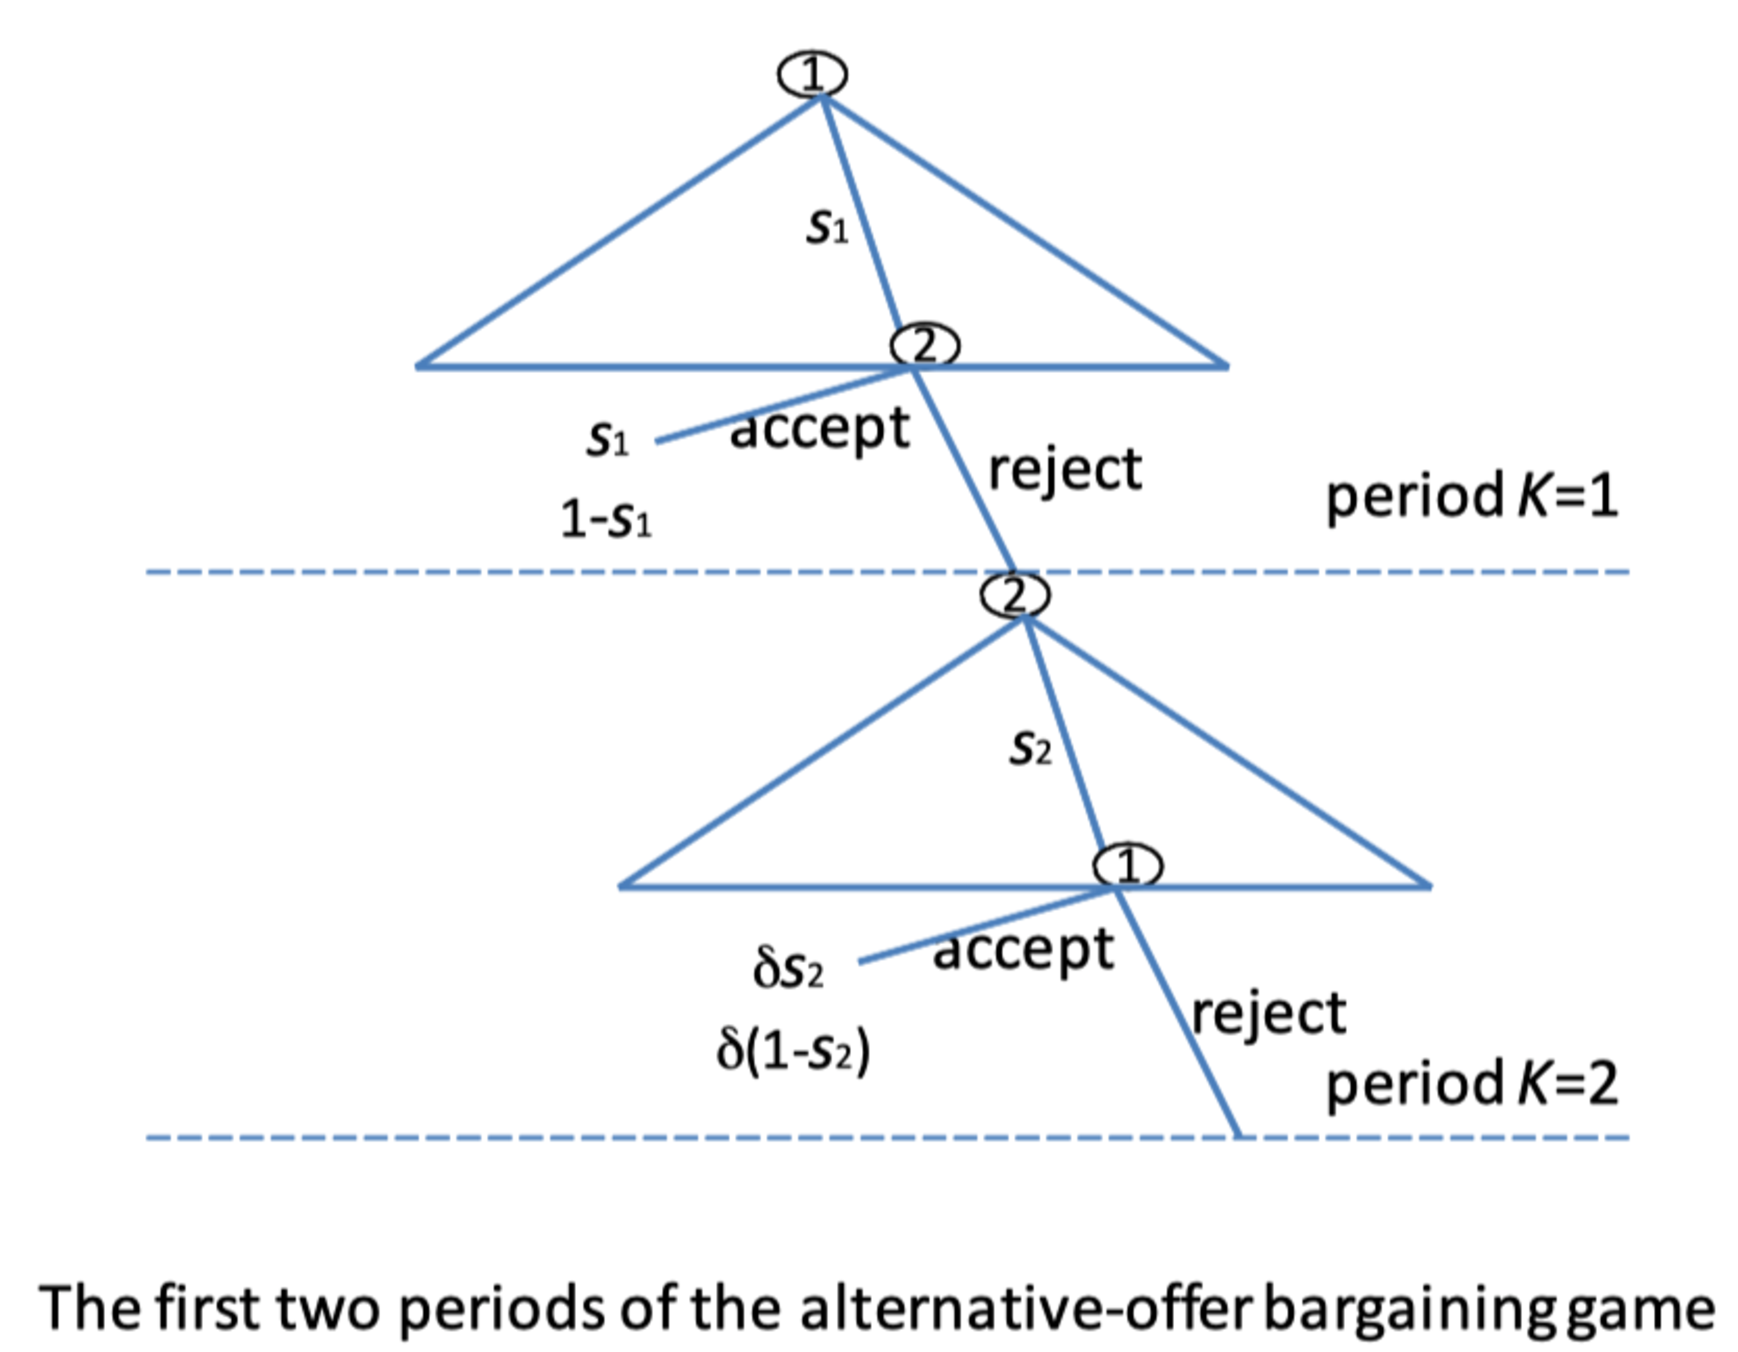
\includegraphics[width=4cm, height=4cm]{bargin_infperiod}\par}
	Note: they are only comparing between this period and next\\

\section{Solving Two-Stage Games of Complete but Imperfect Information}
	Theory: Subgame Perfection

\subsection{Bank run}
	NE: \\
	1. (withdraw, withdraw), \\
	2. [(don't, don't), (withdraw, withdraw)]\\
	date 1
	\begin{tabular}{r|cc}
				&	withdraw		&	don't\\
		\hline
		withdraw	&	40,40		&	50,30\\
		don't		&	30,50		&	next stage
	\end{tabular}\\
	date 2
	\begin{tabular}{r|cc}
				&	withdraw		&	don't\\
		\hline
		withdraw	&	100,100		&	150,50\\
		don't		&	50,150		&	100,100
	\end{tabular}\\
	work backwards: solve for date 2, then date 1


%\subsection{Tariffs and Imperfect International Competition}
%	yet to play
%
%\subsection{Tournaments}
%	yet to play
%
%\section{Solving Repeated Games of Complete but Imperfect Information}
%	Consist of Two-Stage Repeated Games and Infinitely Repeated Games
%
%\subsection{Collusion between Cournot Duopolist}
%	yet to play
%
%\subsection{Efficiency Wages}
%	yet to play
%
%\subsection{Time-Consistent Monetary Policy}
%	yet to play
%
%\section{Solving Dynamic Games of Complete but Imperfect Information}
%	Using concept: Extensive-Form Representation of Games, Subgame-Perfect Nash Equilibrium

%\section{Solving Static Games of Incomplete Information}
%\section{Solving Dynamic Games of Incomplete Information}

\end{multicols}
\end{document}
